\documentclass[fleqn,12pt]{article}
\usepackage{setspace,url,fullpage,latexsym,amsmath,amsthm,amssymb,natbib,graphicx,appendix,float,rotating,caption, subcaption,multirow,longtable,colortbl,xcolor,graphics,graphicx,enumitem,pdflscape,epstopdf,hyperref}
\hypersetup{
	backref =       true,
	pagebackref  =  true,
	colorlinks =    true,
	linkcolor =     blue,
	citecolor =     blue,
	urlcolor =      blue,
}
\bibliographystyle{apsr}
\usepackage[utf8]{inputenc}
\setlength{\tabcolsep}{3pt}										
\singlespacing
\graphicspath{{../figures/}}

\title{Response Memo for ``A Wiki-based Dataset of Military Operations with Novel Strategic Technologies (MONSTr)''}
\date{March 2023}

\begin{document}
\thispagestyle{empty}
\setcounter{page}{0}

\maketitle

We sincerely thank the reviewers and editor for their insights and comments. Responding to the feedback has greatly improved the dataset and manuscript. Accordingly, we have made revisions to accommodate the constructive criticisms detailed below. We have organized our response memo by theme, as (to our delight) there was much agreement among the reviewers about suggested revisions. Most sections include 1) a brief summary of suggested changes and all feature 2) verbatim editor/reviewer comments in italics and 3) a description of changes made, including manuscript extracts where appropriate.

\tableofcontents

\clearpage

\section{Clarify definitions and operationalizations of military interventions, operations, and strategy (R1, R2, R3, \& Editor)}

\noindent \textbf{Author summary of suggested changes:} Two reviewers and the editor observed shortcomings in our discussion and application of MONSTr's unit of analysis that made the dataset's structure difficult to understand. Our unit of analysis needed to be clarified, particularly concerning the size threshold as it related to IMI and MIPS definitions and the definitional coverage of drone strikes. The editor urged us to address these points and precisely outline our unit of analysis. \\

\noindent
\textit{Editor: R2 and R3 emphasize the need for clarity in your definition and your operationalization of military intervention. The unit of analysis needs to be outlined precisely.}

\textit{On the absence of a troop size threshold for interventions noted by R3, looking to the definition provided by the older IMI collection may be valuable since it also has no troop threshold and seems consistent with the present project.} \\

\noindent
\textit{R1: [B]ecause the coding rules include no restriction on the minimum size of the event coded, I would like to know more about the events that may be missing from the data for idiosyncratic reasons. For instance, the data include some drone strikes, but apparently not all of them. If there are more inclusive lists of drone strikes--as I believe there are--it would be useful to know how many of these events wound up in this dataset.} \\

\noindent
\textit{R2: The term military strategy is used too loosely. At times, for example, the authors use the term “military strategy” when referring to the modes of force used in an operation. However, military strategy is much more than just which weapons platforms deliver firepower.} \\

\noindent
\textit{R3: The major issue is that there is no meaningful conceptual or operational definition of an ‘intervention’ or an ‘operation’ that is consistently applied across all cases. More specifically, the authors discuss their criteria on pages 5-6 and begin by comparing their approach to MIPS. MIPS requires “the official deployment of at least 500 regular military personnel to attain immediate term political objectives through action against a foreign adversary” (Sullivan and Koch, 2009, 3). The authors state that they do not include a size threshold for their data. Further, they allow for interventions to have military, rather than political objectives. In addition, they also allow for CIA drone strikes. As a result of the loosening of the definition, it is difficult to say what is an intervention and what is not. It seems that any purposeful application of military or armed force in a foreign territory would count. The authors really need to clarify and state their definition clearly, and demonstrate that it has been consistently applied.}

\textit{The authors also use military ‘interventions’ and military ‘operations’ interchangeably. These are not the same things.} \\

We took these critiques very seriously. One of the authors scoured academic, practitioner, and military publications and consulted with several military personnel (including an individual who contributed to the authorship of the June 2022 update to US Military Joint Publication (JP) 3-0, Joint Operations) to refine and justify our unit of analysis as the military operation. Building upon military definitions from JP 3-0 and the Department of Defense (DoD) Dictionary, we assert that there are meaningful differences between the strategic, operational, and tactical levels of warfare. Although these boundaries are blurry in practice, military doctrine applies these conceptual levels and we cite several academic sources that follow suit and affirm the framework.

Our dataset features military operations that fall within military interventions, events conceptualized and collected at the strategic level. Indeed, the generation of the original Wiki list we scraped stemmed from interventions identified in existing reputable datasets. Our previous efforts to explicitly define military interventions that coincide with MIPS and IMI's approach are now better framed as the identification criteria for what constitutes the sample of military interventions that we dimensionalize to the operational level. Thus, we are still interested in purposeful political uses of force against a foreign adversary, omitting cases that some datasets code as interventions that feature threats, training exercises, routine movements, diplomatic evacuation operations, humanitarian and disaster relief, accidents and non-combat rescue efforts (i.e., cave rescues). Ultimately, the definition we assert for our unit of analysis is about scoping operations within appropriately identified interventions. We combine 1) the gold standard of the DoD definition of a military operation within 2) the scoping conditions of how we define an intervention per MIPS and IMI. We detail this on pages 5 and 6 of the revised manuscript, concluding with our formal definition:

    \begin{quote}
    \textit{A series of tactical actions (battles, engagements, strikes) conducted by combat forces in an operational theater to achieve strategic or campaign objectives in the context of a political issue or dispute through action against a foreign adversary. Routine military movements and operations without a defined target like military training exercises, the routine forward deployment of military troops, non-combatant evacuation operations, and disaster relief are excluded.}
    \end{quote}

Finally, during our operation identification process (see revision item 2) and detailed drone data comparisons (see revision item 5), we eliminated the two drone strikes that were definitively conducted by the CIA--the 2006 Damadola strike and the 2009 Makeen strike, both in Pakistan--since our refined unit of analysis implies that MONSTr exclusively covers DoD-directed drone activity.

More generally, R3 noted that we use military interventions and operations interchangeably despite that these are not the same things. Our comprehensive reworking of our unit of analysis has eliminated this. In the updated manuscript, we refer to interventions as events at the strategic level and operations at the operational level, as defined in the DoD dictionary and JP 3-0 on Joint Operations and reflected in several academic works. We are also careful to distinguish studies and datasets capturing interventions from ours, which disaggregates interventions into individual operations.

R2 also contended that we use the term ``military strategy" too loosely, sometimes as a synonym for the types of force used in an operation. This reviewer rightly pointed out that strategy includes, but is more than mere means of force deployed. We have combed through the manuscript to ensure that we do not conflate strategy and means of force in our prose. The only place where the connection is more pointed is in the beginning of the ``Means of Force" subsection on page 15 where we quote Hart's (1967) definition of military strategy as ``the art of distributing and applying military means to fulfill the ends of policy” (335). To sell the value of having more granular measures of the means of force in our dataset, we emphasize that this is an important \textit{component of} strategy in the manuscript.

\section{Clarify the data's nested structure (R1, R2, R3, \& Editor)}

\noindent \textbf{Author summary of suggested changes:} All reviewers and the editor urged us to more clearly delineate the relationships between operations, their ``parents," and sub-operations. R1 wondered if Wikipedia's raw structure and ``part of" coding is reliable to appropriately nest each event into broader levels, encouraging us to check the events by hand. R2 also challenged the assumption that the most disaggregated event in Wikipedia's structure is necessarily at the operational level, and raised questions about battles or smaller operations within largescale operations. Indeed, military doctrine depicts the operational level of warfare as composed of campaigns and operations suggesting there is nuance even beyond disaggregating to the operational level. R3 noted that we allow for interventions within an intervention, pointing to Figure 3 featuring the Gulf War, its three broad campaigns, and the 26 ``leaf nodes" within it. This reviewer called for clear criteria for what is and is not an intervention to justify such a count. \\

\noindent
\textit{Editors: the relationships among larger or "parent" operations and sub-operations must be clearly delineated.  Similarly, the relationship between "leaf nodes" and criteria in wikipedia and the data generated must be more fully discussed and explained.} \\

\noindent
\textit{R1: I wonder if Wikipedia is sufficiently consistent in its "part of" coding to provide a reliable sense of the broader campaigns within which each use of force is nested. This is probably also something that could be checked by hand once the events are identified.} \\

\noindent
\textit{R2: The structure of the dataset, in particular, the unit of analysis, is hard to understand. The authors state that the unit of analysis is the “military intervention ‘leaf’ node” in Wikipedia. Elsewhere, they imply that “interventions” or “operations” are the unit of analysis. What constitutes an “operation”? Can we really assume that the leaf nodes are all at the operation level? If I understand correctly, what constitutes an observation in the dataset is determined by the somewhat arbitrary level of disaggregation of an event in Wikipedia– i.e., events become disaggregated into multiple leaf nodes as Wikipedia contributors create subentries to existing entries. If so, are the units actually comparable? Do we know that all events that meet the criteria for being an operation are captured in Wikipedia? Is a battle the same as an operation?   When there are operations within operations (e.g., Operation Vigilant Warrior within Operation Southern Watch) – are there observations for the lower-level events and the “parent” event in the dataset? Is there time between these lower-level events that is not captured in any observation in the dataset because it does not have a separate Wikipedia entry? Because the unit of observation in the dataset is so important for determining the usefulness of the data, it is critical that the authors clarify these points. While the authors claim that the dataset “extends breadth by improving the precision” of the unit of analysis (p. 12), I am not convinced of the precision of the units.}

\textit{Including a table with the value of key variables (modes of force, start and end dates, duration, geocoded location, days into parent, ally count, etc…) for all the observations in one major “parent” intervention could be helpful to the reader.} \\

\noindent
\textit{R3: The authors also allow for interventions within an intervention. For example, Figure 3 shows the data on the Gulf War and has 26 leaves. As discussed in the paper, this means the US conducted 26 interventions as part of the Gulf War. What is the criteria used for saying something is and is not an intervention in this case? It seems that these 26 interventions could just as easily be 52 or 13. While there is value in distinguishing phases or operations within a broader intervention, there should be clear criteria for doing so.} \\

We carefully considered these points and took R1's advice to check events by hand. We performed independent audits--one author using an automated approach and one performing manual checks--to ensure that all observations remaining in the dataset reflect military operations. In the ``Clustering - Dependencies and Levels" subsection on pages 12 and 13 of the manuscript, we explain this process as follows:

    \begin{quote}
    \textit{Since MONSTr delves into the operational level, we regarded a particular urgency to capture the higher levels in which each observation is situated. For each case, Wikipedia identifies a ``part of" variable that indicates the broader event to which the former is a subset...This Wikipedia feature enables us to identify and code the campaign and strategic levels in which each operation ought to be nested. To accomplish this, we constructed a dendrogram of the entire dataset, the trunk being any US military intervention in our time period and each branch being an increasingly intricate disaggregation from strategic to operational to tactical levels. We then independently and manually audited all 491 lines to cull operations, paring events at the tactical level, ensuring definitional accuracy, and validating ancestors.}
    \end{quote}
    
    [continues]
    
    \begin{quote}
    \textit{Notably, Wikipedia page names are not always an indication of the event level. They sometimes represent military designations and sometimes public labels. Technically, wars contain campaigns, which contain operations, which contain battles. In Wiki terminology, some entries entitled ``Operation” are not operations according to the DoD definition, some events bearing names like ``Battle of” are operations, and at times operations are nested within campaigns that are labeled as battles. For instance, Operation Euphrates Shield is a broader campaign containing four operations featuring alternative labels, like the East Aleppo Offensive (2017) described as a military operation to capture the Islamic State stronghold of Dayr Hafir and gain control of the city’s water source and airbase. As another example, the Battle of Panjwaii is a two-phase campaign to withstand Taliban forces in the district composed of two operations—Zahara and Medusa. Similarly, the RDF labels for ``instance of" abide by the same nomenclature inconsistencies and cannot be used to determine the case inclusion, which was instead done by the authors.\footnote{For example, Operation Vigilant Sentinel is an instance of ``conflict" while Operation Northern Watch is an instance of ``military operation." For a more thorough evaluation of the scope and relationships of conflict labels in Wikipedia, see (citation redacted).} During our operation identification exercise, we focused on the series of actions and levels of objectives rather than the Wiki names or sizes of events. For any discrepancies, we subjected cases to further scrutiny and debate until reaching consensus.}
    \end{quote}

\section{More mindfully compare with existing datasets (R2, R3, \& Editor)}

\noindent \textbf{Author summary of suggested changes:} Multiple reviewers and the editor requested greater care when comparing MONSTr with existing datasets given variation in temporal and conceptual coverage. The paper needed to clarify how much our expanded \textit{n} is a function of capturing components of cases in existing datasets versus capturing interventions missed by other coders. R3 summarized that our insufficient definitional criteria makes direct comparisons to other datasets complicated, even inappropriate given the granularity of our cases.

\subsection*{Major suggested changes}
\textit{Editor: Multiple reviewers ask for greater care when comparing with existing data sets given variation in conceptual and temporal coverage.} \\

\noindent
\textit{R2: The authors claim to “uncover information about nearly every post-1989 military intervention described in existing academic datasets plus 425 additional operations”.  The 425 additional operations claim is misleading: (1) many of the “additional” operations seem to be components of the cases in existing datasets – i.e., battles, campaigns, or military operations conducted as part of the broader wars/military interventions that are the units of analysis in other datasets, rather than interventions that were missed by other coders. The authors do partially acknowledge this on page 13, but their language elsewhere in the document is misleading. (2) There are only 10-15 years of overlap with 2/3 of the comparison datasets and most of the comparison datasets end prior to the conclusion of the wars in Iraq and Afghanistan. How many of these “additional” operations occur after 2014 or are components of these wars? Are there significant military interventions that are completely missing from other major datasets in years both datasets cover? If so, please give examples and explain why this might be the case.} 

\textit{Moreover, they need to be more careful in their comparisons to other datasets. This dataset has more observations because the observations are more disaggregated.} \\

\noindent
\textit{R3: The lack of clear and consistently applied criteria complicates direct comparisons to other datasets, such as MIP and MIPS, which have very clear conceptual and operational definitions. Yet, the authors make a number of empirical comparisons. For example, “our dataset identifies almost ten times as many events during this period as all existing datasets combined” (p. 2). If I understand correctly, in this comparison the Gulf War counts as 1 intervention, and the 26 interventions within it also count as interventions. It’s just not an appropriate comparison.}

\textit{That said, the data are very interesting and likely very useful for studying military strategies. One path forward is for the authors to use them for this purpose. Possibly use MIP interventions as the unit of analysis, and the Wikipedia data to measure strategies within each intervention. In this way, you’d inherit the conceptual clarity of MIP, but still get the interesting variation in military strategies.} \\

We think that MONSTr's utility is in supplementing, rather than supplanting, existing intervention datasets. To this end, we have significantly shifted the framing of our comparison to existing data, partially as an artifact of clarifying our unit of analysis but also intentionally to situate our contribution more modestly. We removed any verbiage about covering what is missing in other datasets, instead explaining that we are zooming in and providing granularity at the operational level. \\

To accomplish this in a practical sense, we created new variables in MONSTr for ``parent\_X" where X represents each dataset containing military interventions to which MONSTr's operations correspond. In addition to clarifying that MONSTr provides more granular information about the broader interventions described by existing data efforts, this will enable scholars to merge MONSTr to them for myriad analyses. For instance, a researcher interested in what operations and covariates MONSTr captures for just IMI's list of cases, or qualitative scholars performing in-depth analysis on the 12 operations within what MIPS identifies as the ``Kosovo intervention" can now do so with ease.

\subsection*{Minor suggested changes}
\textit{R2: Including a table with the value of key variables (modes of force, start and end dates, duration, geocoded location, days into parent, ally count, etc…) for all the observations in one major “parent” intervention could be helpful to the reader.} \\

During our discussion of the granularity of data coverage on page 14, we direct readers to a new table (Table 1 in the revised manuscript) showing a sample of covariates for some cases in the 2003 Iraq War. \\

\noindent
\textit{R2: Table 2 and Figure one are not useful because observations are based on different units of analysis in each dataset.} \\

We eliminated Table 2 and Figure 1 per R2's sugggestion. With the refined unit of analysis and merging variables, what is now Table 2 in the revised version following the addition of the above table now provides a sufficient comparison of the variables included at different levels of analysis and provides readers with a list of relevant intervention datasets with which MONSTr can interface. \\

\noindent
\textit{R3: It is not true to say that there is an “assumption of independence across cases” in other data projects on military intervention (p. 9). To my knowledge, none of the mentioned datasets claim interventions to be independent of one another. It is true that relations between cases may not be recorded, but that does not mean they are assumed to be independent.} \\

We have eliminated this claim and all mentions of case relationships in existing datasets state that this is a technical trait only.

\section{Detail validation checks more thoroughly (R1, R2, R3, \& Editor)}
\noindent \textbf{Author summary of suggested changes:} All reviewers requested more detail on the verification checks we performed. R1 was keen to know whether we checked events to detect duplicates or problematic observations. The editor agreed with R1's promotion that we perform and report manual checks to ensure the veracity of the data. R2 asked for more detailed information on our manual validation processes of all variables and their nestings. In addition, R2 inquired on which external sources we used to verify the reliability of Wikipedia's information. R3 reinforced these requests, wanting to know the nature of our external sources and to ensure they are not the same as those cited by Wikipedia. \\

\noindent
\textit{Editors: greater detail on your verification checks are required, as R1 and R2 note.  R1 in particular sees value in reporting manual checks to ensure the veracity of the data and we agree.} \\

\noindent
\textit{R1: First, I would like to know whether they checked the coded events to see if there are duplicates or other problematic observations. The dataset is not so large that checking every event is impossible.} \\

\noindent
\textit{R2: The paper should include much more detailed information about how the authors conducted “manual validation” of the values of key variables in the dataset. In particular, the authors need to provide more thorough evidence that Wikipedia’s coding of “means of force used” is accurate, that Wikipedia reliably identifies all battles and operations conducted within a broader campaign/war/intervention, and that the start and end dates for battles and uses of particular means of force are accurate. Which external sources were used to verify the accuracy of Wikipedia’s information? Can you provide statistics on the reliability of Wikipedia coding of the values of key variables?} \\

\noindent
\textit{R3: Would definitely want to see more about how the Wikipedia data was validated. Did the authors use the same sources that were cited for Wiki? They claim data was randomly sampled and checked against external sources (p. 9). What are those external sources? Are they news sources? Government sources?} \\

During the data collection process, we ensured that there are no duplicates in the dataset through a number of techniques: 1) organization by unique Wikidata IDs, 2) data validation tools in our software and code, and 3) manual row-by-row reading of every Wiki page by research assistants overseen by the authors. The additional exhaustive audits we performed as part of our revisions to ensure that only operations comprise our unit of analysis solidified the absence of duplicates and problematic observations.

We have also provided detailed information of the data validation we performed including the cases randomly selected, the sources used to check each one, and our evaluative conclusions. We discuss this on page 11 of the revised manuscript and in the third section of the Appendix. 
    
\section{Provide more information on Wiki inclusion criteria and missingness (R1, R2, \& R3)}
\subsection*{\textit{Inclusion Criteria}}
\textit{R3: The authors could provide a discussion of a how a datapoint gets into the RDF databases in the first place (p.7-8). Is there any sort of review required? Documentation? Discussion? If so, what is it? We know a lot about media coverage of conflict, or at least we know something about it (e.g., Croicu and Eck 2022, Dietrich and Eck 2020). How does Wikipedia compare in terms of making the record?} \\

The original manuscript primarily evaluated wikipedia in terms of its accuracy, but not its inclusion criteria. To make the improvement suggested by the reviewer, the subsection ``Cleaning - Auditing and Validating" has been updated to include a discussion about (1) Wikipedia's inclusion criteria when deciding whether an event should get a Wikipedia page, (2) a summary of existing research on wikipedia's event coverage, including known biases regarding the recency of events and events relevant to English-speaking and Western audiences, (3) a summary of existing research on event datasets and media coverage of conflict, including the cites suggested by the reviewer, and (4) an explanation of coverage biases the authors uncovered in manually examining the observations in MONSTr. \\

\textit{R3: In addition, how does something in the RDF get labeled? For example, looking at Figure 3, some are battles and some are operations. What’s the difference?} \\

The short answer is that whether Wikidata/DBpedia classify a page as an ``instance of" (P31) a ``conflict" or ``military operation" is irrelevant for this paper, as is whether a Wikipedia page name contains the words ``operation," ``battle," etc. Since an academic paper introducing a new dataset on military operations requires a more clear and consistent inclusion criteria than what Wikipedia provides, whether a Wikipedia entry corresponds to a military operation is a coding decision that is made by the authors (as explained above) rather than something decided by RDF labels. Recognizing that others may disagree about what pages we include, our coding decisions are transparent in the replication code and produced in a way where other scholars can change what observation in each branch of the nested tree constitutes the operation-level observation and then rerun the code to see if modeling results differ.

The long answer involves a rather detailed explanation of RDF labeling. Wikidata and DBpedia are organized as triples (subject-predicate-object) where each Wikipedia page (subject) has a list of predicates (properties) with coded values (object). Subjects and objects always correspond to Wikipedia pages and have a unique ID that starts with ``Q". Predicates are the ``edges" (in network terms) that describe the type of connection between the subject and object and have a unique ID that starts with ``P".

For example, the first subject-predicate-object RDF for Nelson Mandela is Q8023-P31-Q5 which means 

\begin{quote}
    ``Nelson Mandela" (subject Q8023) \\
    is an ``instance of" (predicate P31) \\
    ``human" (object Q5). 
\end{quote}

The most important RDF property is ``instance of" (P31). Every time a new page is created, the originator must decide of what that page is an instance. R1's question about Resource Description Framework (RDF) labeling can refer to either (1) what predicates (properties) are provided for each page or (2) what object (value) is provided. To be comprehensive, we explain the labeling process for both.

\subsubsection*{RDF predicate labeling}
Once the page creator assigns an ``instance of" classification, Wikidata has a template that provides a list of other suggested properties that are likely relevant for that category. So once Nelson Mandela is assigned an ``instance of" of P5 (human), Wikidata prompts entry of other common properties like sex or gender (P21), country of citizenship (P27), and date of birth (P569). In some cases, predicates differ across pages even when they are identical for our purposes. For example, some pages have a variable from the RDF predicate ``start time" (Property:P580) while others have the RDF predicate ``inception" (Property:P571).

In terms of R3's question about how something in the data structure is labeled, the first answer is that the predicate labels are determined by a combination of the ``instance of" Wikidata template and other predicates are chosen manually by page editors. The predicate labels are then filtered by the authors (us) based on relevance\footnote{Not all RDF predicates are included in our data. For example, the ``Barisha raid" operation that killed al-Baghdadi has a property for ``named after" (P138) with a value of ``Kayla Mueller." Kayla Mueller was a US aid worker who had been killed by the Islamic State. While interesting, the ``named after" predicate exists for very few observations and is thus omitted. However, the replication code that will become publicly available would allow other scholars to add predicates to our original SPARQL query if they wished.} and combined/aggregated where appropriate.

\subsubsection*{RDF object labeling}
R1's example of battles vs operations gets to the second element concerning how something in the data structure gets labelled -- the labeling of the RDF \textit{object}. Despite that we just made the case that the most important RDF is ``instance of" (P31), we largely ignore it. There are over 100,000 possible P31 values on Wikidata/DBpedia that are not mutually exclusive and do not necessarily align with how political scientists think of those terms.

The authors find the question about what ``instance of" label a page is assigned so interesting, however, that it is the subject of another paper by one of the authors that examines all ``conflicts" on Wikipedia and their types/subtypes. An illustrative example from the author's other paper is shown in Figure \ref{fig:p13}. A cite to this (unpublished working) paper is omitted in the current MONSTr submission to adhere to double-blind anonymization, but would be included in an accepted manuscript.

\begin{figure}[h]
    \begin{center}
	\caption{Wikidata ``instance of" labels for existing conflict dataset pages}
	\label{fig:p13}
	{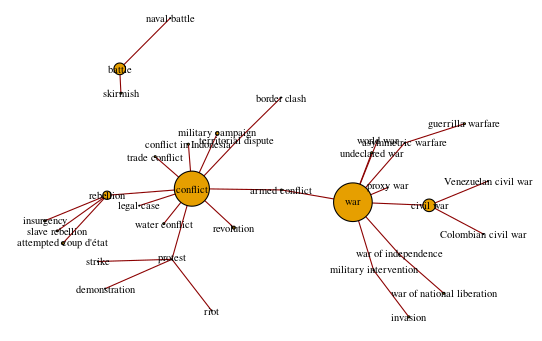
\includegraphics[width = \textwidth]{conflict_branch_existingdata.png}}
    \end{center}
\end{figure}

But we digress. How do the observations \textit{in MONSTr} get labeled? Matching all IMI observations to their corresponding Wikidata pages, for example, results in 13.9\% having an ``instance of" (P31) value of ``war" (Q198), 9.8\% having ``conflict" (Q180684), 6.4\% having ``civil war" (Q8465), 5.9\% having ``military operation" (Q645883), etc. On the one hand this is encouraging, as we would expect more observations in IMI to be instances of ``war" (P198) than ``superhero" (Q188784).\footnote{154 and 0, respectively.} On the other hand, Operation Vigilant Sentinel (Q7097689) is an instance of ``conflict" (Q180684) while Operation Northern Watch (Q2026233) is an instance of ``military operation" (Q645883). Why? The short answer is we don't know. We hope the working paper mentioned above can (eventually) figure that out. In the meantime, this paper sets aside the type of event identified by Wikipedia (``instance of") and instead decides what observations to include in MONSTr manually based on our definition of a military operation. The discussion of our refined definition in sections 1 and 2 of the response memo outlines the process by which we did this.

The paper also ignores the terminology and word choice in the Wikipedia page name for the same reason. The page for ``1993 cruise missile strikes on Iraq" (Q5189962) does refer to an event that meets our definition of a military operation while the page for ``Operation Enduring Freedom" (Q326668) does not. After coding the full nested tree of every Wikipedia entry that is a part of any US military intervention, we identify the leaf on each branch that meets our definition of the operation-level unit of analysis as defined and explained at the beginning of this response memo.

\subsection*{\textit{Missingness}}
\textit{R2: Do we know that all events that meet the criteria for being an operation are captured in Wikipedia?} \\

The simple answer is no, Wikipedia does not capture an exhaustive list of military operations. It does, however, capture events that reach a certain threshold of public attention, interest, and demand. We think this is theoretically important and interesting. Especially with increasingly fragmented and polarized information environments in American news media that generate and sustain ``echo chambers," Wikipedia remains a frequently consulted source for information on political and military events across political spectrums. This makes MONSTr somewhat akin to an events dataset (news article = Wiki page) resting on highly attractive features of Wiki--dramatically broader audience than single news outlets, objective data point orientation, scrapable structure. \\

We also delved into the detailed answer. Although missingness is a perennial problem in international relations data, we have aimed to identify the direction and extent of it in MONSTr not only relative to existing datasets but also to the theoretical universe of relevant cases. Of the former, the original manuscript focusing on MONSTr's coverage in comparison to extant military interventions datasets demonstrated that Wiki, and therefore we, capture every observation within our criteria covered elsewhere. Thus, in comparison to standing scholarly resources on military interventions, MONSTr has no missingness. \\

Equally meaningful, we appreciate the reviewers' challenge to address missingness relative to data beyond US military interventions (i.e., drone strikes datasets). To examine our coverage of drone strikes, we consulted the reputable and rather comprehensive Bureau of Investigative Journalism (BIJ) database.\footnote{Bureau of Investigative Journalism. 2020. "Drone Warfare." \textit{Bureau of Investigative Journalism.} \href{https://www.thebureauinvestigates.com/projects/drone-war}{https://www.thebureauinvestigates.com/projects/drone-war}.} Its coverage is more focused than New America, Long War Journal, Institute for the Study of Counterterrorism and Unconventional Warfare, and Airwars which often conflate drone and air strikes (at times even ground raids). It is worth noting that most datasets on drone strikes are sharply focused on the opaque CIA program conducted in non-war zones. We are pursuing a fundamentally different sample focused on military operations. Indeed, we removed the two CIA-operated drone strikes from the dataset during our military operations identification exercise. Other databases also focus solely on kinetic strikes while we consider reconnaissance uses in support of operations as well. Nonetheless, comparing coverage is valuable to identify and explain the overlap. BIJ covers drone strikes in Afghanistan (2015--2020), Pakistan (2004--2018), Somalia (2007--2020), and Yemen (2002--2020). Aggregating them to the country-year for comparative overview, Table \ref{tbl:drones} overwhelmingly illustrates that BIJ covers far more. At the same time, MONSTr includes some strikes that BIJ, focusing primarily on the CIA program, does not. \\

\begin{table}
    \caption{Comparison of US Drone Strike Incidents}
    \label{tbl:drones}
    \centering
    \begin{tabular}[h]{|lcc|}
    \hline
    \textbf{Country} & \textbf{BIJ} & \textbf{MONSTr} \\
    \hline
        Afghanistan & 14,079 & 5 \\
        Iraq & - & 6 \\
        Libya & - & 1 \\
        Pakistan & 430 & 6 \\
        Somalia & 191 & 3 \\
        Syria & - & 3 \\
        Yemen & 326 & 4 \\
    \hline
    \end{tabular}
\end{table}

Among the four nations of common coverage, we scrutinized the cases that made it into MONSTr to identify what might explain why they, of all others, exist on Wikipedia. The first factors are salience and sensationalism. The types of drone strike events that earn their own Wiki page involve targeted killings of major military targets (i.e., the successful 2020 strike on Iranian general Qasem Soleimani) or major condemnation on grounds of collateral damage and humanitarian norms (i.e., the 2006 Chenagai strike allegedly targeting al-Zawahiri but decimating a madrassa, killing 82 civilians including children and teachers, and motivating mass protests). Indeed, drone strikes are inherently, intentionally more covert than other means of force, persisting undetected at medium to high altitudes, escaping many aerial defense systems' target acquisition algorithms due to their slower flight paths, and most being quieter than cruise missiles and manned craft (especially stealth models). Consequently Wiki rarely captures drone strike events unless they rise on the public awareness radar in their aftermaths. This is admittedly a bias in MONSTr, but one we accept on the logic of building a type of events dataset centered on publicly known military operations. \\

The second factor affecting inclusion is based on our definitional design and code. We capture events having their own Wikidata ID / Wikipedia page so that we can scrape appropriate covariates. Short of being quite newsworthy, most individual drone strikes (those performed independently of a combined arms military operation) are cataloged on Wiki pages as mere lists with no hyperlinks to individual events or information beyond an indication that they occurred, such as \href{https://en.wikipedia.org/wiki/List_of_drone_strikes_in_Afghanistan}{this one}. We do not include these in MONSTr due to the dearth of information on them.

\section{Explain the absence of naval interventions (R1)}
\textit{R1: Finally, the authors note on page 16 that "[b]y our definition of intervention, we do not observe any naval interventions within our time scope." I find this statement puzzling. The definition of intervention given on page 5 explicitly includes naval actions. If the data collection procedure somehow did not find any of them, I would like to know why.} \\

We revisited all observations in MIPS and IMI (the only two featuring naval means) that are coded as naval interventions. We then identified 1) whether that observation exists in our dataset given a match with a Wikipedia page via Wikidata Qcode, 2) if that observation meets the inclusion criteria for our refined definition of a military operation per revision item 1 above, and 3) what military means are coded for it in MONSTr. Through this process, we validated that our dataset does not feature any cases that merit the coding of naval means for two reasons. First, some interventions coded as naval are outside the scope of our definition as humanitarian or disaster relief events.

Second, for the remainder of mutual cases our coding divergence hinges on the way the naval vessels were used. When a cruise missile is launched from a naval vessel, IMI and MIPs code it as naval while MONSTr codes it as a ``cruise missile" means. Similarly, when aircraft take off from a naval vessel to perform an aerial bombing mission we code this as an ``aerial bombing" means. We are agnostic about the launch points or service branch of these platforms, instead capturing the administration of means. The sole other case featuring naval means refers to the method of conveyance of ground troops to the island of Haiti, which we code as ground troops. For transparency, we detail these cases for both datasets below and have created a new document in the replication data and repository with more complete tables and code.

Additionally, we have revised the text that (rightfully) puzzled R1. We clarify at the end of the ``Means of Force" subsection that 

\begin{quote}
    \textit{Although some intervention datasets identify naval events during this time period, those events are identified in MONSTr by how the target was attacked, rather than the launch point (ie cruise missiles launched from a destroyer are coded as cruise missiles and an island landing for a raid is coded as ground troops). We explain this choice and our divergence from all cases coded as naval elsewhere in detail in the Appendix, allowing scholars to recode relevant cases in MONSTr as naval if desired.}
\end{quote}

\noindent
We then summarize the points outline in this response memo and include the detailed comparisons below in the Appendix. As an aside, R1's comment has prompted us to think about how version 2.0 of MONSTr could capture the military services participating in each operation. It has certainly sparked our interest, but it is beyond the coding we have done to this point.

\subsection*{\textit{IMI naval interventions}}
IMI contains 19 observations coded as naval means. All have corresponding Wikipedia pages. Of those, ten do not meet our criteria for inclusion in MONSTr as humanitarian or disaster relief operations. They include (as listed in IMI): 

\begin{quote}
    \textit{US troops give humanitarian relief to Somalia (Xinh, UP, AP) \\
    Operation Assured Response by US to evacuate 2444 people from Liberia (globalsecurity.org) \\
    US evacuates American citizens from Albania (GNL) \\
    US evacuates civilians from Sierra Leone (DP, Xinh) \\
    US send peacekeepers to Liberia (Fed. Info, AFP, DP) \\
    US provides tsunami relief to Thailand (AP, BBC) \\
    US provides tsunami relief to Indonesia (FT, AFP, Scripps) \\
    US provides tsunami relief to Sri Lanka (AFP, AP) \\
    US troops build schools and provide medical aid in Haiti (AP, Navy Newsstand) \\
    US evacuates American citizens from Liberia during civil conflict (CSM, AP, WP)}
\end{quote}

Of the remaining nine naval cases, three are coded as naval ``shelling," four as naval ``intimidate," and two as naval ``transportation." All ``shelling" cases are coded in MONSTr as cruise missile cases, and additional checks confirm that the nature of naval involvement was solely as the origin of the missile launch. Of the four ``intimidate" cases, three concern Operations Desert Storm and Desert Shield, where the naval intimidation involved repositioning vessels that were later used to launch cruise missiles or aircraft. Those three are coded in MONSTr as cruise missile and aerial bombing cases. The remaining ``intimidate" case is 

\begin{quote}
    \textit{US restores democratically elected government in Haiti (UPI, AP)}
\end{quote}

\noindent
which MONSTr codes as ground troops and paramilitary since their conveyance to the theater was the purpose of the vessel's presence. The remaining two ``transport" cases are 

\begin{quote}
    \textit{US buildup of troops in Kuwait after Iraq's provocation (SDUT, Reuters) \\
    US aids in restoring order in Haiti (AP, AFP)}
\end{quote}

\noindent
both of which MONSTr codes as ground troops for the same reason as the last.

\subsection*{\textit{MIPS naval interventions}}
MIPS has 33 observations coded as naval means. Twenty-four were determined outside the definitional criteria for inclusion in MONSTr because they were humanitarian or disaster relief operations or militarized events that, in our minds, did not constitute a US military intervention (e.g., observations ``Fishing Boats," ``Evacuating U.S. citizens," ``Venezuelan Refugees Humanitarian mission," and ``Detention of U.S. Service members").

The remaining nine populate on Wikipedia and are thus included in MONSTr. MIPS does not code the type of naval intervention like IMI does, instead featuring a binary variable indicating presence and a ``MaxNavy" variable corresponding to the number of vessels. Eight of these cases are coded in MONSTr as cruise missiles or bomber aircraft, launched from naval vessels. The sole case in our dataset that does not correspond to an aerial launch point from a naval vessel is Operation Uphold Democracy, which is the same 1991 Haitan coup attempt that IMI codes as a naval ``intimidate" and that we code as ground troops.

\section{Justify the absence of parent fixed effects in the demonstrative model (R2)}
\noindent \textit{R2: These results of the preliminary analysis are interesting. Two main concerns: The authors argue that their dataset allows analysts to account for strategic dependencies based on strategic campaign and parent-intervention fixed effects, but they do not do this in their example analysis. Instead, fixed effects are at the president level. Why?} \\

We realized from this that we failed to articulate in the manuscript that our models do capture the ancestor nestings of the operations. Rather than including them as fixed effects in a logit model, we ran hierarchical models that require specification of which variables capture the nested structure. We have corrected this at the end of the first paragraph under the ``Specification" subsection on page ENTER, now reading:

\begin{quote}
    \textit{The dependent variables are binary and the data are nested, calling for a logit estimator in hierarchical models that account for the strategic dependencies of operations within wars.}
\end{quote}

\noindent
\textit{R2: Second, and relatedly, it would be helpful to know how many of the 326 observations in the analysis are events that take place within Operations Iraqi Freedom and Enduring Freedom.} \\

Of the 313 military operations in our dataset, 93 occur during OIF and 90 occur during OEF. Many of the rest occur within the Syria Civil War, Gulf War, OEF -- Horn of Africa, and Kosovo War. As mentioned in revision item 3 above, the dataset now features columns indicating each operation's intervention ancestor as featured in existing datasets to allow users to isolate operations as desired, such as those in OIF and OEF.

\clearpage
\setstretch{1.0}

\end{document}